\documentclass[a4paper, 12pt]{article}
\usepackage[utf8]{inputenc}

%=== Packages ===%

% German language encoding
% \usepackage[ngerman]{babel}
% \usepackage[utf8]{inputenc}
% \usepackage[T1]{fontenc}

% decrease caption size
\usepackage{caption}
\captionsetup{font=footnotesize}

% chess board
\usepackage{xskak}

% multiple footnotes
\usepackage[multiple]{footmisc}

% add graphics
\usepackage{graphicx}

% graphics next to each other
\usepackage{subcaption}

% used for custom enumarations
\usepackage{enumerate}
\usepackage[shortlabels]{enumitem}

% improved tabular package
\usepackage{tabularx}

% for hyperlinks
\usepackage[hidelinks]{hyperref}

% Bibliography/Citations
\usepackage{cite}
\usepackage{natbib}

% Draw Pictures
\usepackage{tikz}

\usepackage{ifthen}

% Glossary
\usepackage[acronym, toc]{glossaries}
\makenoidxglossaries
\newglossaryentry{Board State}{
	name={BoardState},
	description={Describes the positions of the pieces on the chessboard at a given time (Equivalent to the term position)}
}

\newglossaryentry{DeepBlue}{
	name={DeepBlue},
	description={First chess engine to win against a world chess champion}
}

\newglossaryentry{Stockfish}{
	name={Stockfish},
	description={Most use free and open source Sachach engine}
}

\newglossaryentry{threats}{
	name={threats},
	description={A move that attacks the opponent in such a way that they are forced to react so that they do not suffer a disadvantage}
}

\usepackage{acronym}

%=== Document Setup ===%

% set margin
% use 2cm at the top if no header is used
% use 2.5cm at the bottom if fotter is used
\usepackage[left=3cm, right=2cm, top=2.5cm, bottom=2cm]{geometry}

% headline
\usepackage{fancyhdr}
\usepackage{enumitem}
\usepackage{amsmath}
\usepackage{amssymb}

\pagestyle{fancy}
\fancyhf{}
\rhead{Page \thepage}
\lhead{Generating Chess Commentary using Machine Learning}
% \cfoot{}

% for inline code blocks
\usepackage{listings}
\usepackage{xcolor}

\definecolor{backcolour}{RGB}{245, 245, 245}

\lstdefinestyle{codestyle}{
	backgroundcolor=\color{backcolour},
    commentstyle=\color{gray},
    numberstyle=\ttfamily\scriptsize,
    basicstyle=\ttfamily\footnotesize,
    breakatwhitespace=false,         
    breaklines=true,                 
    captionpos=b,                    
    keepspaces=true,                 
    numbers=left,                    
    numbersep=5pt,                  
    showspaces=false,                
    showstringspaces=false,
    showtabs=false,                  
    tabsize=2,
    % xleftmargin=0.15in
}

\lstset{style=codestyle}

\begin{document}

\newgeometry{left=2.5cm, right=2.5cm, top=2.5cm, bottom=2.5cm}

\begin{titlepage}
% University Informations
\begin{flushleft}
Frankfurt University of Applied Sciences\\
Fachbereich 2: Informatik und Ingenieurwissenschaften\\
Informatik (B.Sc.)\\
\end{flushleft}

\vspace{3.5cm}

% Thesis Title
\begin{center}
\Large
\textbf{Creating virtual chess commentators using neural networks}\\
%\large
Subtitle
\end{center}

% Abstract
\begin{abstract}
Computer generated move analysis has become an essential part of today's chess world. This scientific work deals with the question of how neural networks can be used to analyze chess games and create a virtual chess commentator. In particular, we will look at what is needed to represent a chess board that can be used by the neural network to plan and compare moves in order to make an appropriate evaluation of a game of chess. Based on this, we will then explore how the neural network can convert the evaluation into natural language that humans can understand.
\end{abstract}

\vspace{6cm}
	
% Lecturer Informations
\begin{flushright}
Lecturer: Konstantin Ernst\\
Course: Künstliche Intelligenz und wissenschaftliches Arbeiten\\
Winter Semester 22/23\\
\end{flushright}

\vspace{2cm}

% Your Informations
\begin{flushleft}
Submitted by:\\
Max Semdner\\
Matrikelnr.: 1294899\\
\href{mailto: max.semdner@stud.fra-uas.de}{max.semdner@stud.fra-uas.de}\\
\end{flushleft}

\end{titlepage}

\newpage

% Abstract
\begin{abstract}
This scientific seminar paper deals with the question how machine learning can be used to generate comments on chess games. On the one hand it is shown how a chess engine can be built to analyze games and on the other hand how the information provided by the engine can be used by a virtual chess commentator to generate comments. The engine is built based on a neural network and a Monte-Carlo Tree Search algorithm and can be trained by self-play. The generation is based on an encoder-decoder model that uses a bidirectional long short-term memory architecture. For a total of five different categories, comments are generated by corresponding generation models, which together form the virtual chess commentator.
\end{abstract}
\addcontentsline{toc}{section}{Abstract}


\restoregeometry

\tableofcontents

\newpage

\section{Introduction}

In the mid-20th century, computer chess experienced its first breakthroughs thanks to the work of scientists like Alan Turing, Claude Shannon and John von Neumann. Alan Turing, the pioneer of artificial intelligence, was convinced that games were an ideal model system for machine learning.\footnote{Cf. \cite{levy-newborn-1982}, pp. 44-45} This prediction has come true, and machine learning have proven to be an essential part of many chess engines today. In particular, recent projects such as AlphaZero, developed by DeepMind, show how efficient programs which use neural networks are in analyzing board games compared to traditionally used algorithms such as alpha-beta search.\footnote{See \cite{alphazero-2018}, p. 1} Although chess engines have become a powerful tool, they have a lack of transparency regarding the moves they perform. Therefore, professional chess players and commentators are often needed to explain the intention of these moves. This dependence on human chess commentators can be a disadvantage, since moves found by computers can sometimes be misinterpreted or not understood at all. Especially for non-professional chess players, many moves played by humans as well as computers are incomprehensible, since they do not have the appropriate experience. In the following, the construction of a chess engine is discussed, which corresponds in its play and analysis strength to the engines of today. This should serve to analyze moves in their depth. Then the construction of a virtual chess commentator is described, which uses the information gained by the analysis of the chess engine to create detailed comments on a given position and move.

\section{Generating Chess Commentary}

% \subsection{General Approach}

% \subsubsection{General Approach}

The chess commentator has the task of translating certain information, which it receives from the chess engine described before, into human understandable comments. Such a task falls into the domain of \textit{sequence-to-sequence} processing. The idea of sequence-to-sequence models is to map an input of a certain length to an output of a certain length, where input and output length can be different.\footnote{Cf. \cite{Sutskever-2014-sts}, p. 1} For such tasks, encoder-decoder architectures with attention has achieved great success in the past. An architecture proposed by \cite{zang-etal-2019-automated} consists of two parts, an encoder and a decoder, which are two \textit{bidirectional recurrent neural networks (Bi-RNN) using long short-term memory (LSTM) state cells}.

Recurrent neural networks (RNN) are neural networks designed to process sequences of data. RNNs process the data sequences in a time-dependent manner by putting the generated outputs back into the network along with new inputs.\footnote{Cf. \cite{rnn-2015-review}, p. 2} This allows the network to remember ongoing patterns in the data and respond to those patterns. State and time are related in recurrent networks because the reused output and the newly added input adjust the values in the RNN accordingly.\footnote{Cf. \cite{rnn-2015-review}, p. 8} The state in the network, therefore, represents the values of the neurons in the network at a given time. Bidirectional recurrent neural networks are a special type of recurrent networks that consider both the previous and subsequent input data, unlike traditional RNNs that consider only the previous input data.\footnote{Cf. \cite{https://doi.org/10.48550/arxiv.1801.01078}, p. 1} This is done by splitting "the state neurons of a regular RNN in a part that is responsible for the positive time direction (forward states) and a part for the negative time direction (backward states)"\footnote{\cite{Schuster1997BidirectionalRN}, p. 2674}. This enables them to remember and respond to ongoing patterns in both directions along the sequence. One problem of RNNs and Bi-RNNs is the processing of long input sequences, where the so-called "vanishing gradient problem" can occur, whereby the network is no longer able to correctly consider the information from the past. This can be solved by recurrent networks that use a long short-term memory architecture. LSTM cells are special neurons that allow the network to remember and respond to ongoing patterns over long periods of time.\footnote{Cf. \cite{rnn-2015-review}, p. 17} This makes them particularly well suited for processing sequences where patterns persist over an extended period of time.

\begin{figure}[h]
\centering
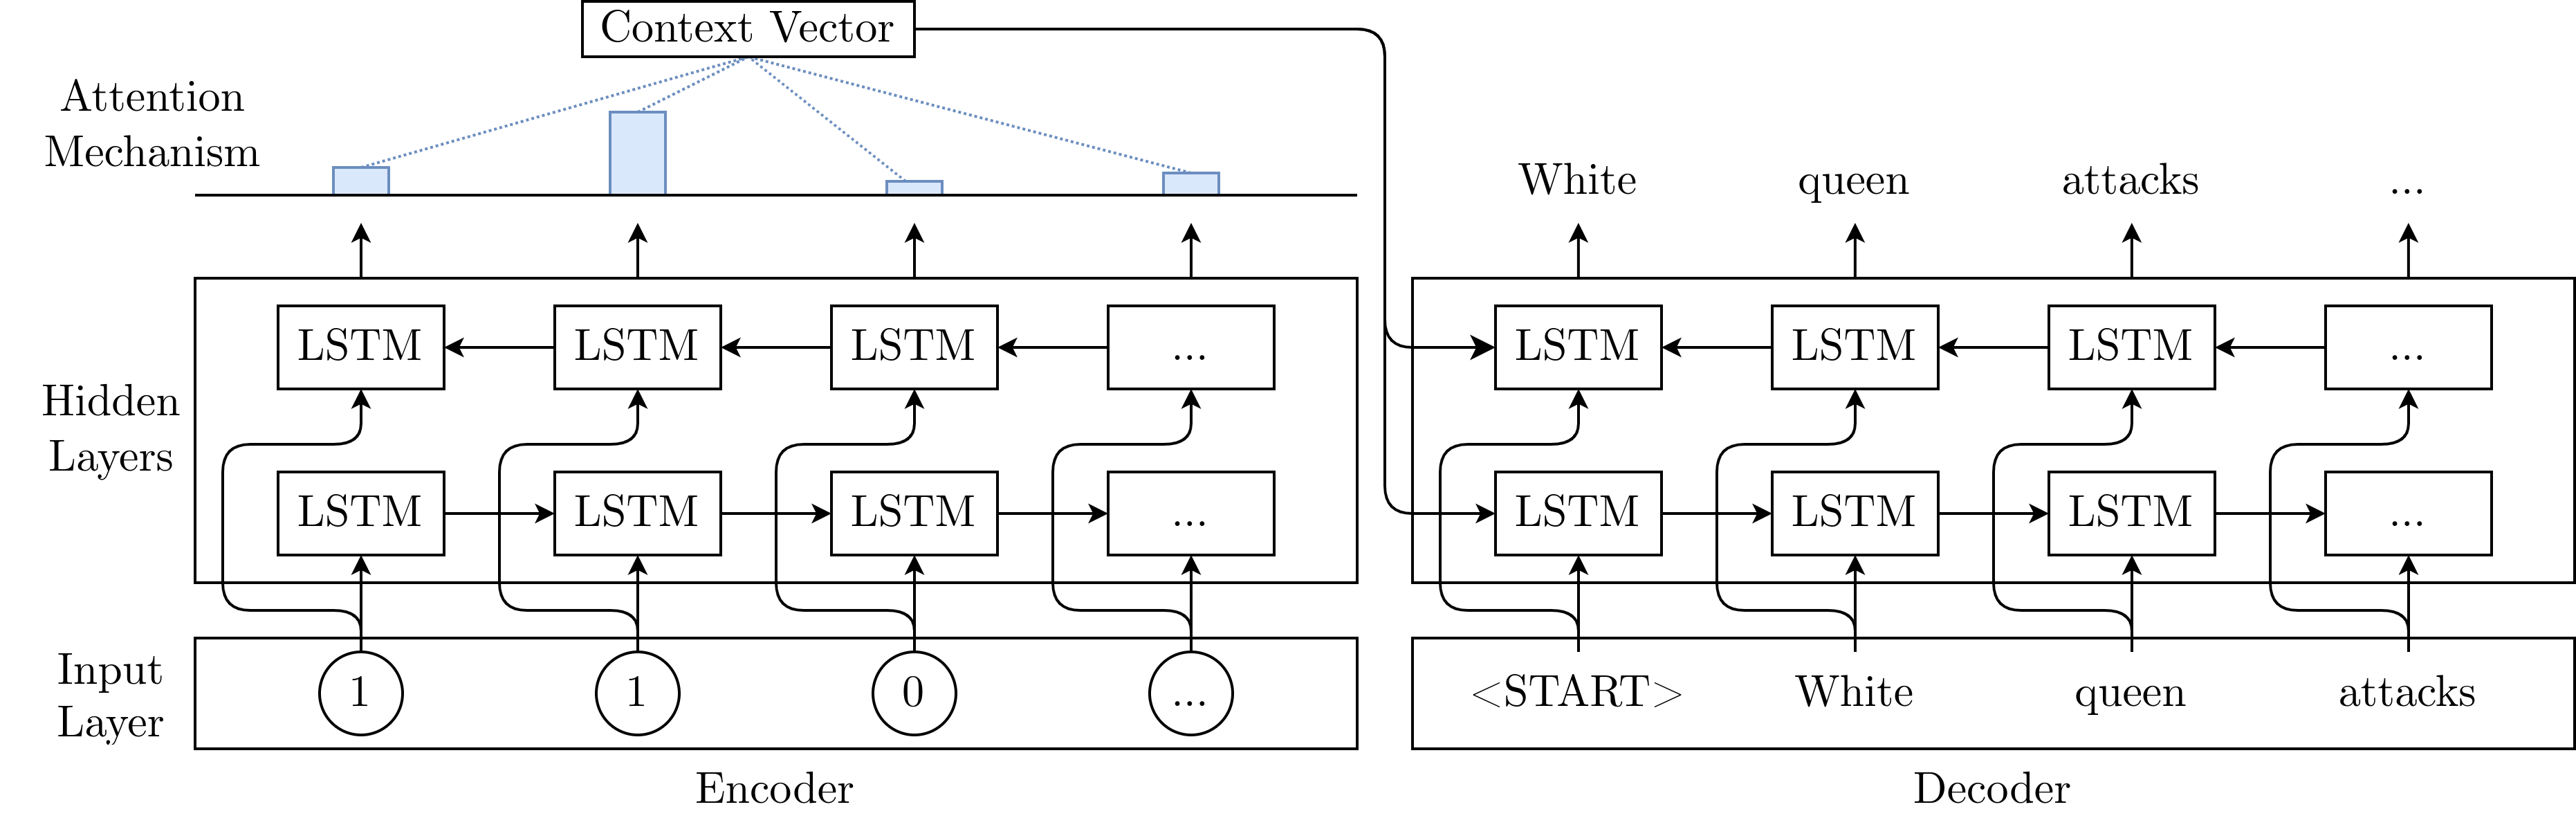
\includegraphics[width=\textwidth]{graphics/commentator_example/general_approach.png}
\caption{Chess Commentator Encoder-Decoder Architecture with Attention Mechanism (Note: Figure based on \cite{jhamtani-etal-2018-learning} Figure 4)}
\label{fig:eda}
\end{figure}

The encoder-decoder architecture used for generating chess commentary makes use of the described Bi-LSTMs.\footnote{Cf. \cite{zang-etal-2019-automated}, p. 2}  It’s a model used in machine translation and other areas of artificial intelligence. It consists of two main components: the encoder and the decoder. The encoder is responsible for converting the input into an appropriate representation (e.g., a vector of numbers). The decoder uses this representation to produce the desired output.\footnote{Cf. \cite{https://doi.org/10.48550/arxiv.1406.1078}, p. 1} In the case of the chess commentary translation the encoder receives a sequence of data, generated by the chess engine (position and move), processes the data and encodes it  into a "fixed-length vector representation"\footnote{\cite{cho-2014-ende}, p. 1}. This vector are the last states of the encoder. The vector can either be used as initialization for the LSTM cells of the decoder or as additional input for each step of the generation of the output.\footnote{Cf. \cite{mohajerin-2017-state}, pp. 1-2} One problem that affects the quality of the decoder’s translation, is the length of the sequences. The sequence stored in the vector tends to dilute over time, resulting in poor translations. To solve it, an attention mechanisms can be used. The attention mechanism allows the decoder to "selectively focusing on parts of the source"\footnote{\cite{luong-2015-attention}, p. 1} while producing the desired output. This is done while processing the data in the encoder, which encodes only the most important information in the vector, called the context vector. It can be said that the context vector contains a summary of the sequence. This allows the decoder to focus only on the information relevant for translation. If the decoder now wants to generate comments, it receives a start symbol as input (represented by \texttt{<START>} in Figure \ref{fig:eda}). This start symbol is used to indicate the start of the output sequence. The first output is the first word of the translation. The output is additionally used as new input in the next step, generates an output and which is used as the new input again. This procedure is repeated until an end symbol is reached, which signals the end of the sequence. The generated output sequence is the translation, so here the chess comments.

\subsection{Chess Engine}

\subsubsection{Requirements}

Any chess engine must meet a number of requirements in order to function. These requirements include the \textit{representation of the chessboard}, the \textit{search of the possible moves} and the \textit{evaluation of the position}.\footnote{Cf. \cite{nnfc-2022}, pp. 75-76} These requirements can be implemented in a number of ways. Certain implementation options have become widely accepted. In the following, one implementation procedure is presented in detail for each requirement. These are state of the art implementations that have been in use for many years or have achieved great success in the recent past.

\subsubsection{Board Representation}

Since the computer cannot work with a physical chess board and pieces, these must be converted into a form in which the board, pieces, and position can be interpreted by the computer and later used for the input layer of the neural network. The most common way of representing positions and movements of chess pieces is the data structure bitboards. A bitboard is implemented as an $8 \times 8$ bit array, which is the size of a chessboard.\footnote{Cf. \cite{boskovic-2005-bb}, p. 360} Each array element corresponds to a square on the board. A bitboard is created for each type of piece (pawn, knight, bishop, rook, queen and king) of a given color (black and white). Further 4 board for "2 casteling choices of each player"\footnote{\cite{zang-etal-2019-automated}} are generated. This gives a total number of 16 bitboards. Finally, the squares on which the figures are placed must be marked on the respective boards. This can be done in binary, where 0 means the square is empty and 1 means the square is not empty.

\begin{figure}[h]
\centering
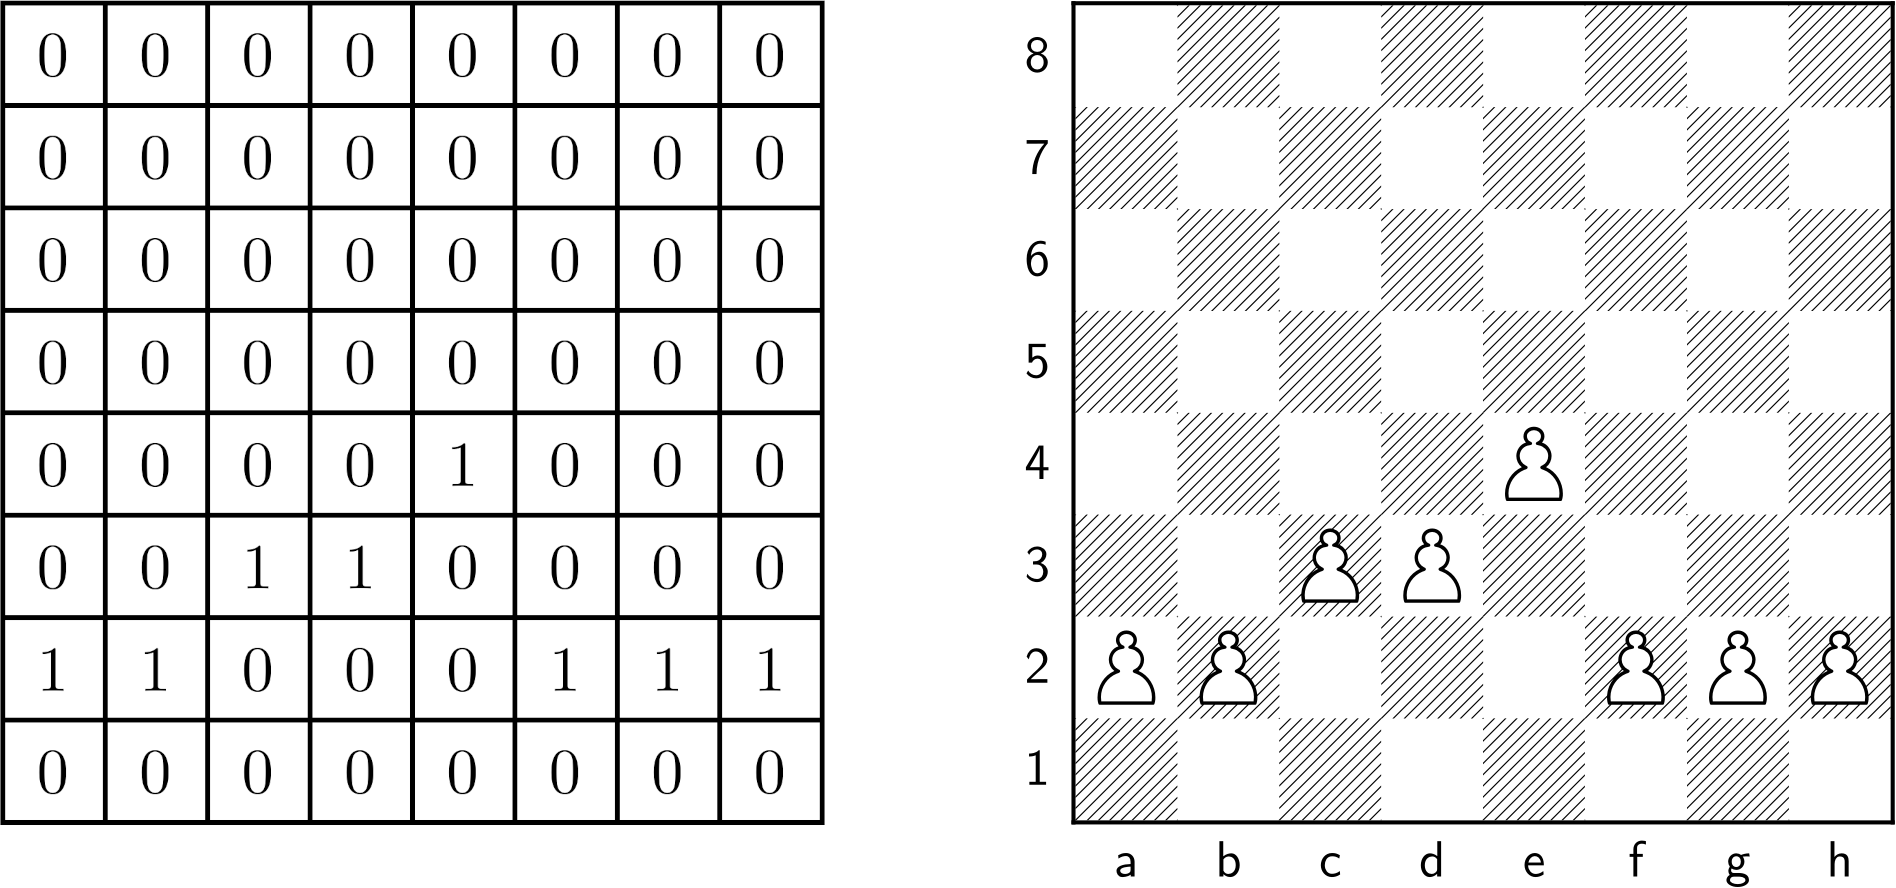
\includegraphics[width=0.5\textwidth]{graphics/bitboard/bitboard_and_chessboard.png}
\caption{Representation of bitboard with white pawns (left) and the corresponding chessboard (right)}
\end{figure}

Bitboards can also be used to represent possible movements of chess pieces. This is achieved by performing certain logical operations on the bitboard. The main advantage of the logical operations are, that they can be executed quite quickly by the processor.\footnote{Cf. \cite{boskovic-2005-bb}, p. 360} Furthermore, with x64 processors the position can be stored in a bit string in the memory, since this is exactly 64 bits long due to the number of squares.\footnote{Cf. \cite{segundo-2005-bb}, p. 67} Another advantage is that it can be used as input for the input layer in the neural network due to its simple representation. The network could then be trained to evaluate specific chess positions and predict moves.

\subsubsection{Move Search and Position Evaluation}

A challenge for both humans and computers is to find the best possible move. In fact, chess is considered unsolved, i.e. it is not known if there is an optimal strategy that always leads to victory, for either sides. The objective of a good chess engine is therefore to find the best move based on its computational capabilities. One factor to consider is the depth of analysis. Thus, each move must be considered not only in terms of the current state of the board, but also what effect it will have on subsequent best moves and positions. In order to find the best move, two tasks must be achieved, one is to find the legal, possible moves in the current and the following positions, and the other is the evaluation of these positions.

To implement these two tasks, many systems such as \Gls{DeepBlue} and earlier versions of \Gls{Stockfish} use human-defined evaluation functions and game tree search algorithms. The evaluation function receives the board as input and evaluates how good the obtained position is. Game tree search algorithms, such as MiniMax, are then used to search for all possible moves (Usually, up to a certain depth, e.g. 15 moves). Each move leads to a new position. Since there is no information about these new positions yet, they need to be evaluated by the evaluation function. In the end, the path that has received the highest value from the evaluation function is chosen. Improvements such as alpha-beta pruning remove paths that are known not to yield high values of the evaluation. The problem with this method is that the evaluation functions have to be written by hand with the help of chess experts and constantly refined to achieve an optimal result.

To overcome this problem, and to get the best results from the engine for the commentator, machine learning is used. \cite{alphazero-2018} presented an algorithm that uses Monte Carlo tree search (MCTS) and a neural network. The neural network is used to evaluate an input position. It outputs two pieces of information: A vector with the move probabilities of all next legal moves and, a value, which tells what the player's chances of winning are for the given position. MTCS is used to search deeper, i.e., to search many possible move paths and then select the path with the best evaluation. To select the next move MCTS selects "each valid move, play a number of random games"\footnote{\cite{nnfc-2022}, pp. 106-107}, generates statistics for these randomly selected paths and compares them.\footnote{See \cite{nnfc-2022}, pp. 100} The best evaluated move of a path is played. The statistical evaluation for each path can be generated by the evaluations made by the neural network at each node of the search tree.

\begin{figure}[h]
\centering
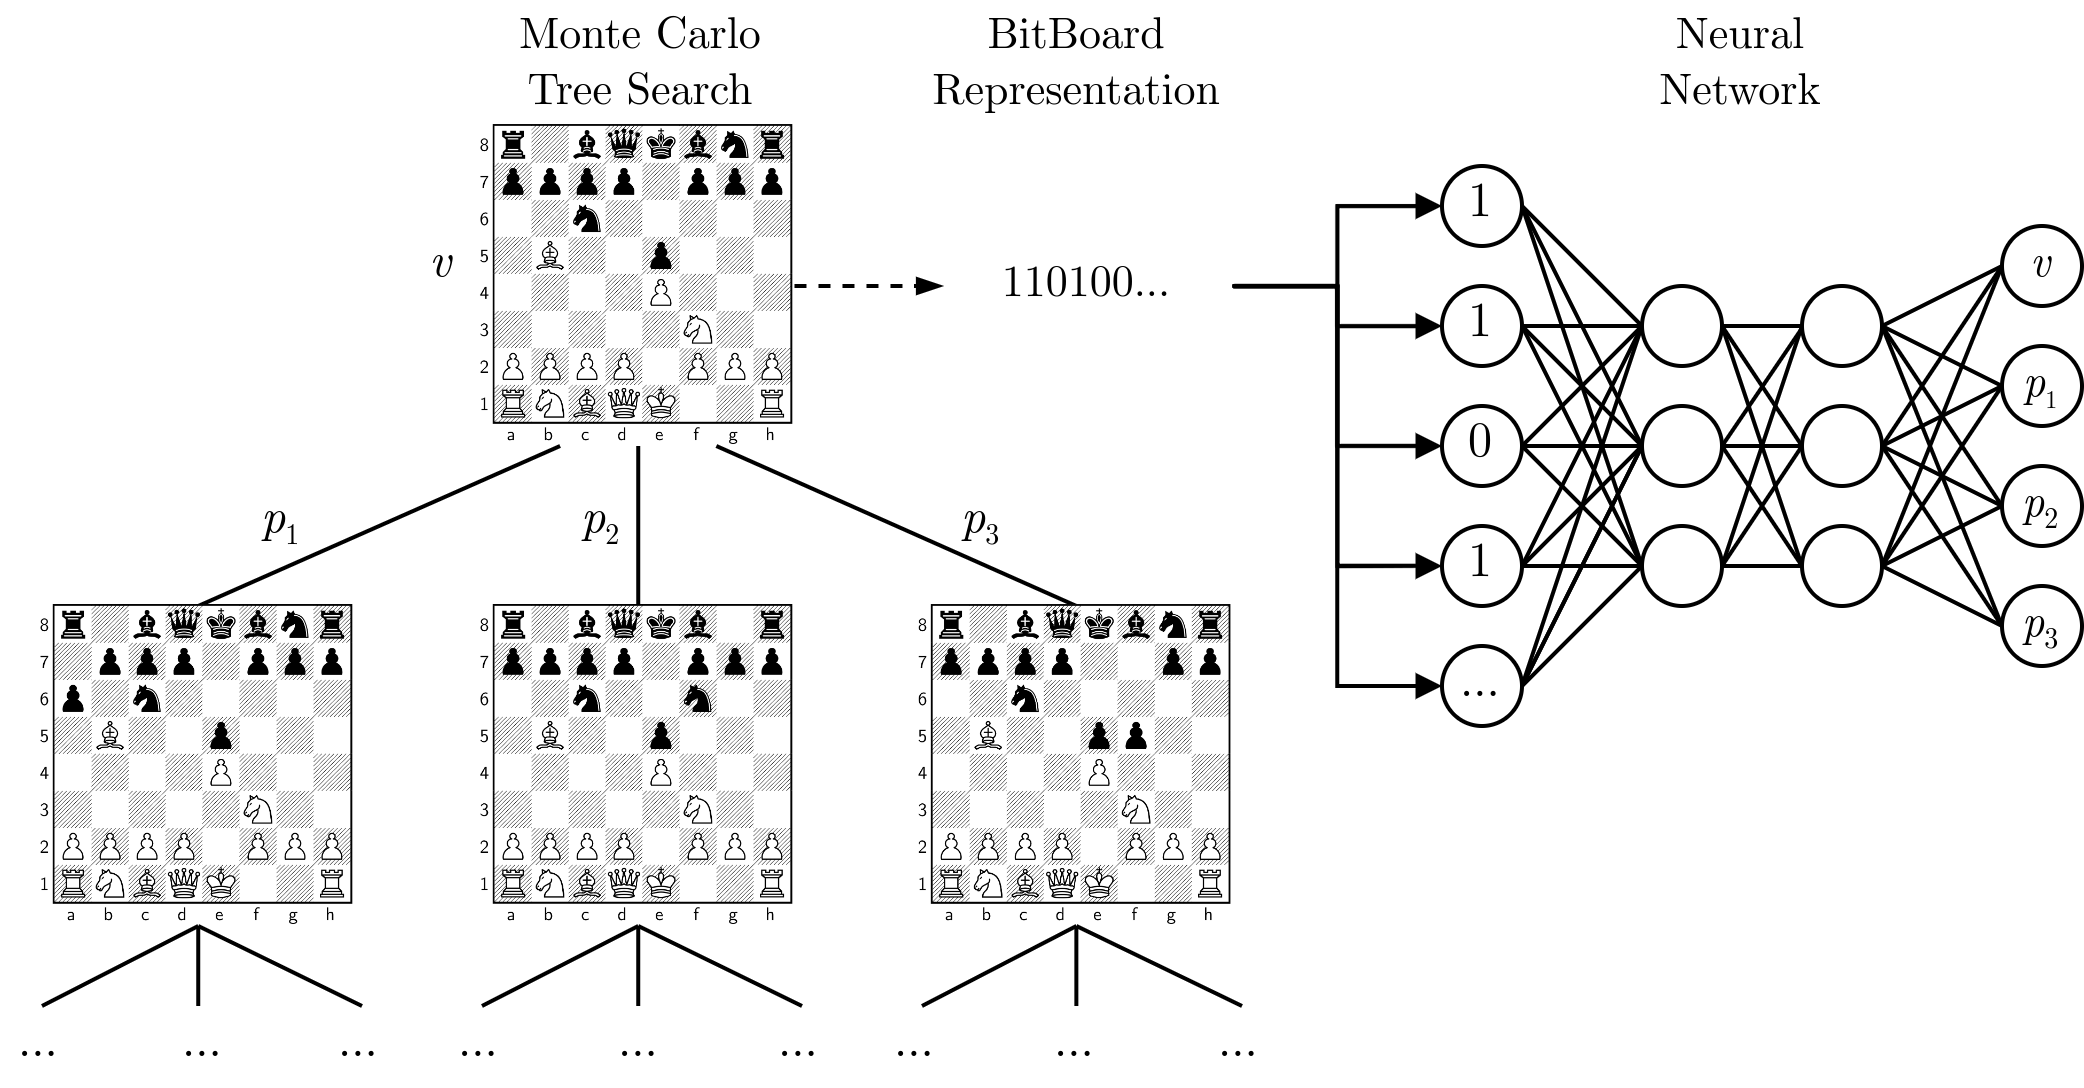
\includegraphics[width=0.95\textwidth]{graphics/alphazero/alphazero.png}
\caption{Simplified example of move search and position evaluation using MCTS and a neural network. ($p_{n}$ move probabilities, $v$ winning chance value)}
\end{figure}

In order for the neural network to deliver the best possible results, it must be trained with data. Instead of relying on existing data sets, \cite{alphazero-2018} used the approach of generating their own data sets through self-play. Initially a program exists that only knows the rules of the game, uses an untrained neural network for evaluation and the MCTS algorithm for move selection. The program executes the following four steps to train the neural network: (1) The program plays against itself by searching for several moves in advance through the MTCS, letting the neural network evaluate these moves for move probability and position strength, and finally choosing the path with the best evaluation. Every game is recorded move by move. At the end of each match, the final position of the sides are assigned lost (-1), drawn (0) or won (+1) to create a dataset.\footnote{See Silver et. al p. 2} (2) The neural network is cloned and the parameters are adjusted "to minimize the error between the predicted result [...] and the game result [...]" and train the network with the generated data set. (3) Let the new program play against the previous one. (4) The winning program is selected and the process is repeated from step 1. As \cite{alphazero-2018}  showed, this method was able to outperform Stockfish, the strongest engine at this time, after only 4 hours.

\begin{figure}[h]
\centering
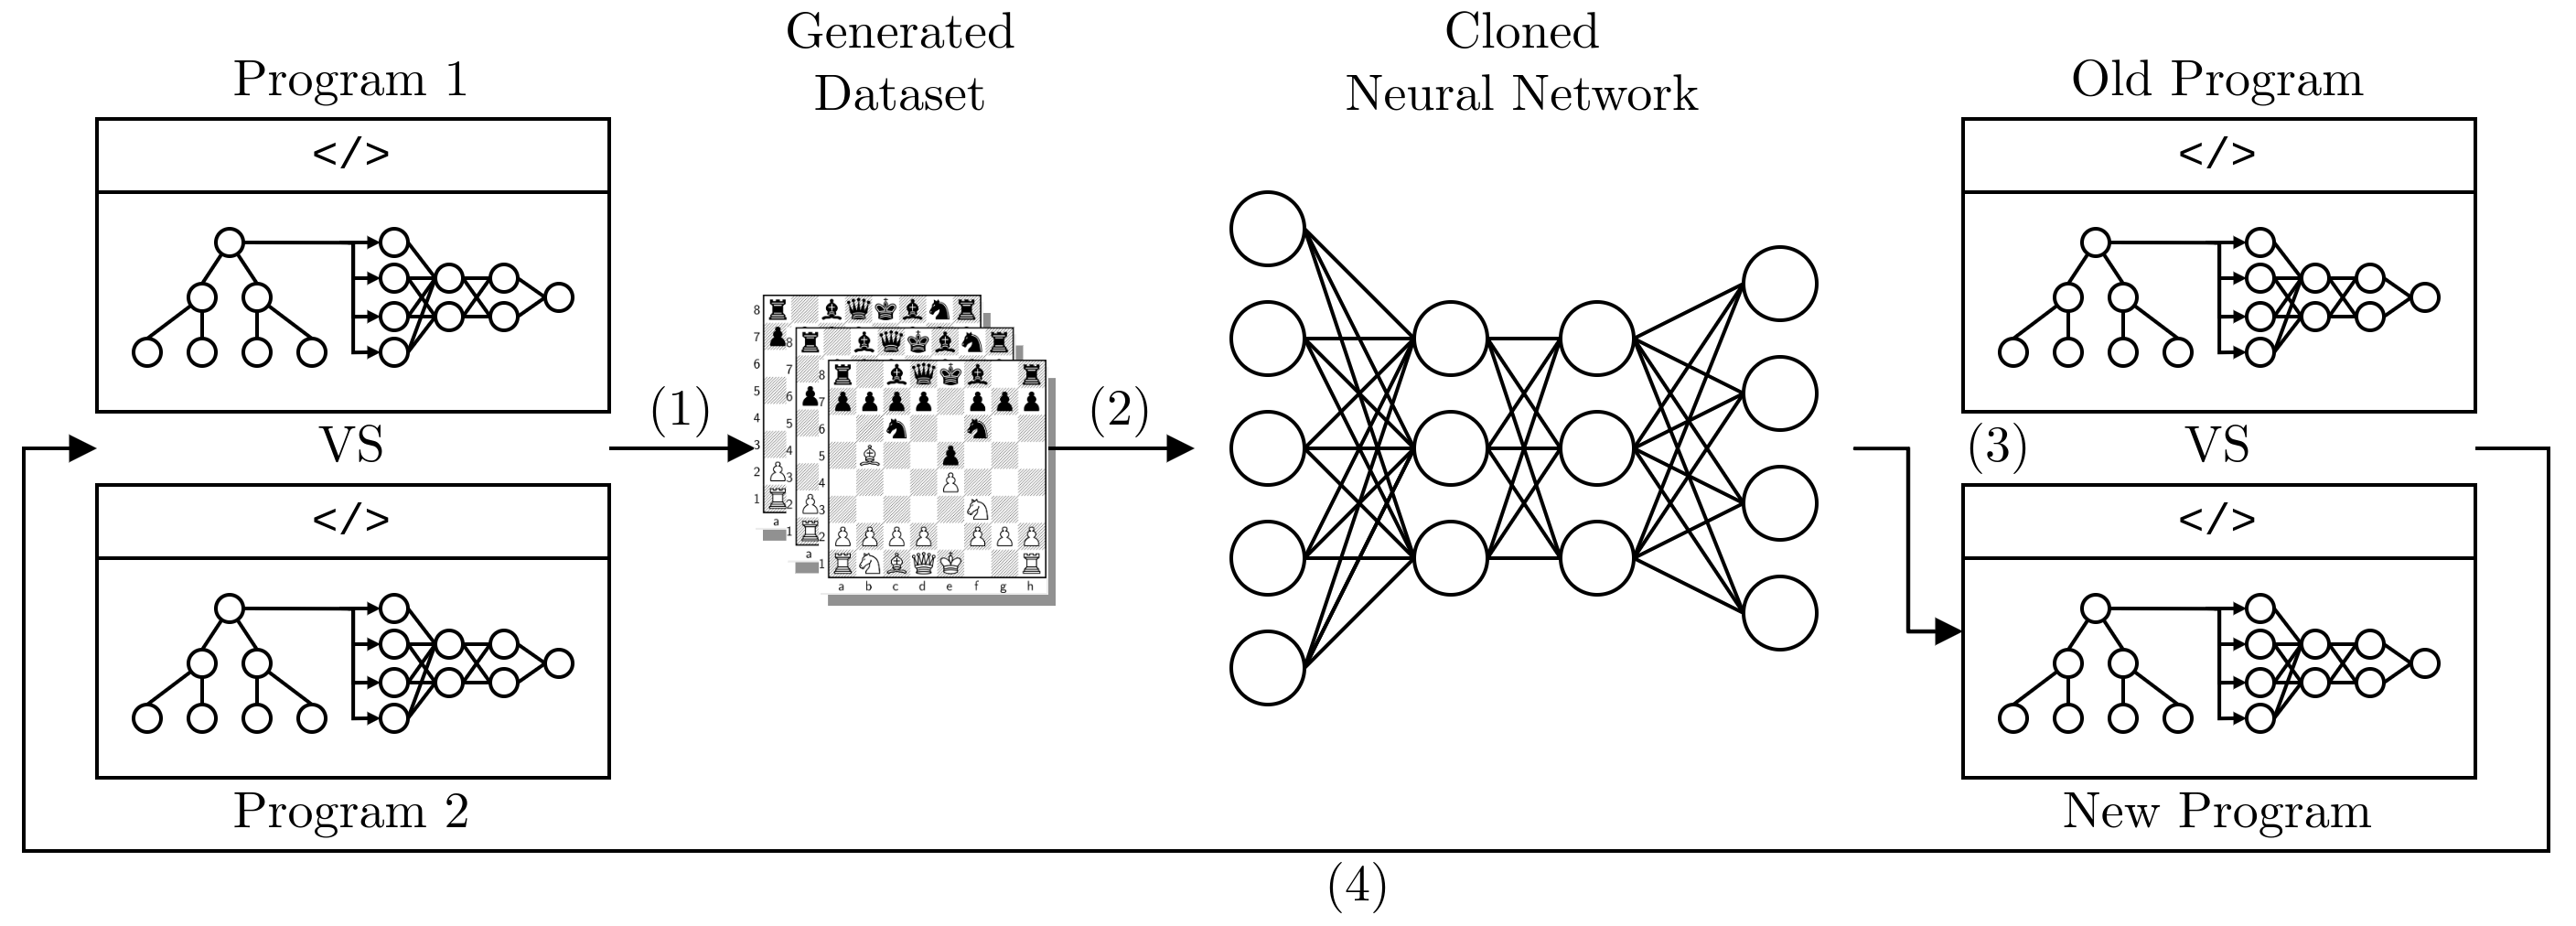
\includegraphics[width=0.95\textwidth]{graphics/alphazero/selfplay.png}
\caption{Steps of traning the neural network through self-play}
\end{figure}

\subsection{Chess Commentator}

\subsubsection{General Approach}

The chess commentator has the task of translating certain information, which it receives from the chess engine described before, into human understandable comments. Such a task falls into the domain of \textit{sequence-to-sequence} processing. The idea of sequence-to-sequence models is to map an input of a certain length to an output of a certain length, where input and output length can be different.\footnote{Cf. \cite{Sutskever-2014-sts}, p. 1} For such tasks, encoder-decoder architectures with attention has achieved great success in the past. An architecture proposed by \cite{zang-etal-2019-automated} consists of two parts, an encoder and a decoder, which are two \textit{bidirectional recurrent neural networks (Bi-RNN) using long short-term memory (LSTM) state cells}.

Recurrent neural networks (RNN) are neural networks designed to process sequences of data. RNNs process the data sequences in a time-dependent manner by putting the generated outputs back into the network along with new inputs.\footnote{Cf. \cite{rnn-2015-review}, p. 2} This allows the network to remember ongoing patterns in the data and respond to those patterns. State and time are related in recurrent networks because the reused output and the newly added input adjust the values in the RNN accordingly.\footnote{Cf. \cite{rnn-2015-review}, p. 8} The state in the network, therefore, represents the values of the neurons in the network at a given time. Bidirectional recurrent neural networks are a special type of recurrent networks that consider both the previous and subsequent input data, unlike traditional RNNs that consider only the previous input data.\footnote{Cf. \cite{https://doi.org/10.48550/arxiv.1801.01078}, p. 1} This is done by splitting "the state neurons of a regular RNN in a part that is responsible for the positive time direction (forward states) and a part for the negative time direction (backward states)"\footnote{\cite{Schuster1997BidirectionalRN}, p. 2674}. This enables them to remember and respond to ongoing patterns in both directions along the sequence. One problem of RNNs and Bi-RNNs is the processing of long input sequences, where the so-called "vanishing gradient problem" can occur, whereby the network is no longer able to correctly consider the information from the past. This can be solved by recurrent networks that use a long short-term memory architecture. LSTM cells are special neurons that allow the network to remember and respond to ongoing patterns over long periods of time.\footnote{Cf. \cite{rnn-2015-review}, p. 17} This makes them particularly well suited for processing sequences where patterns persist over an extended period of time.

\begin{figure}[h]
\centering
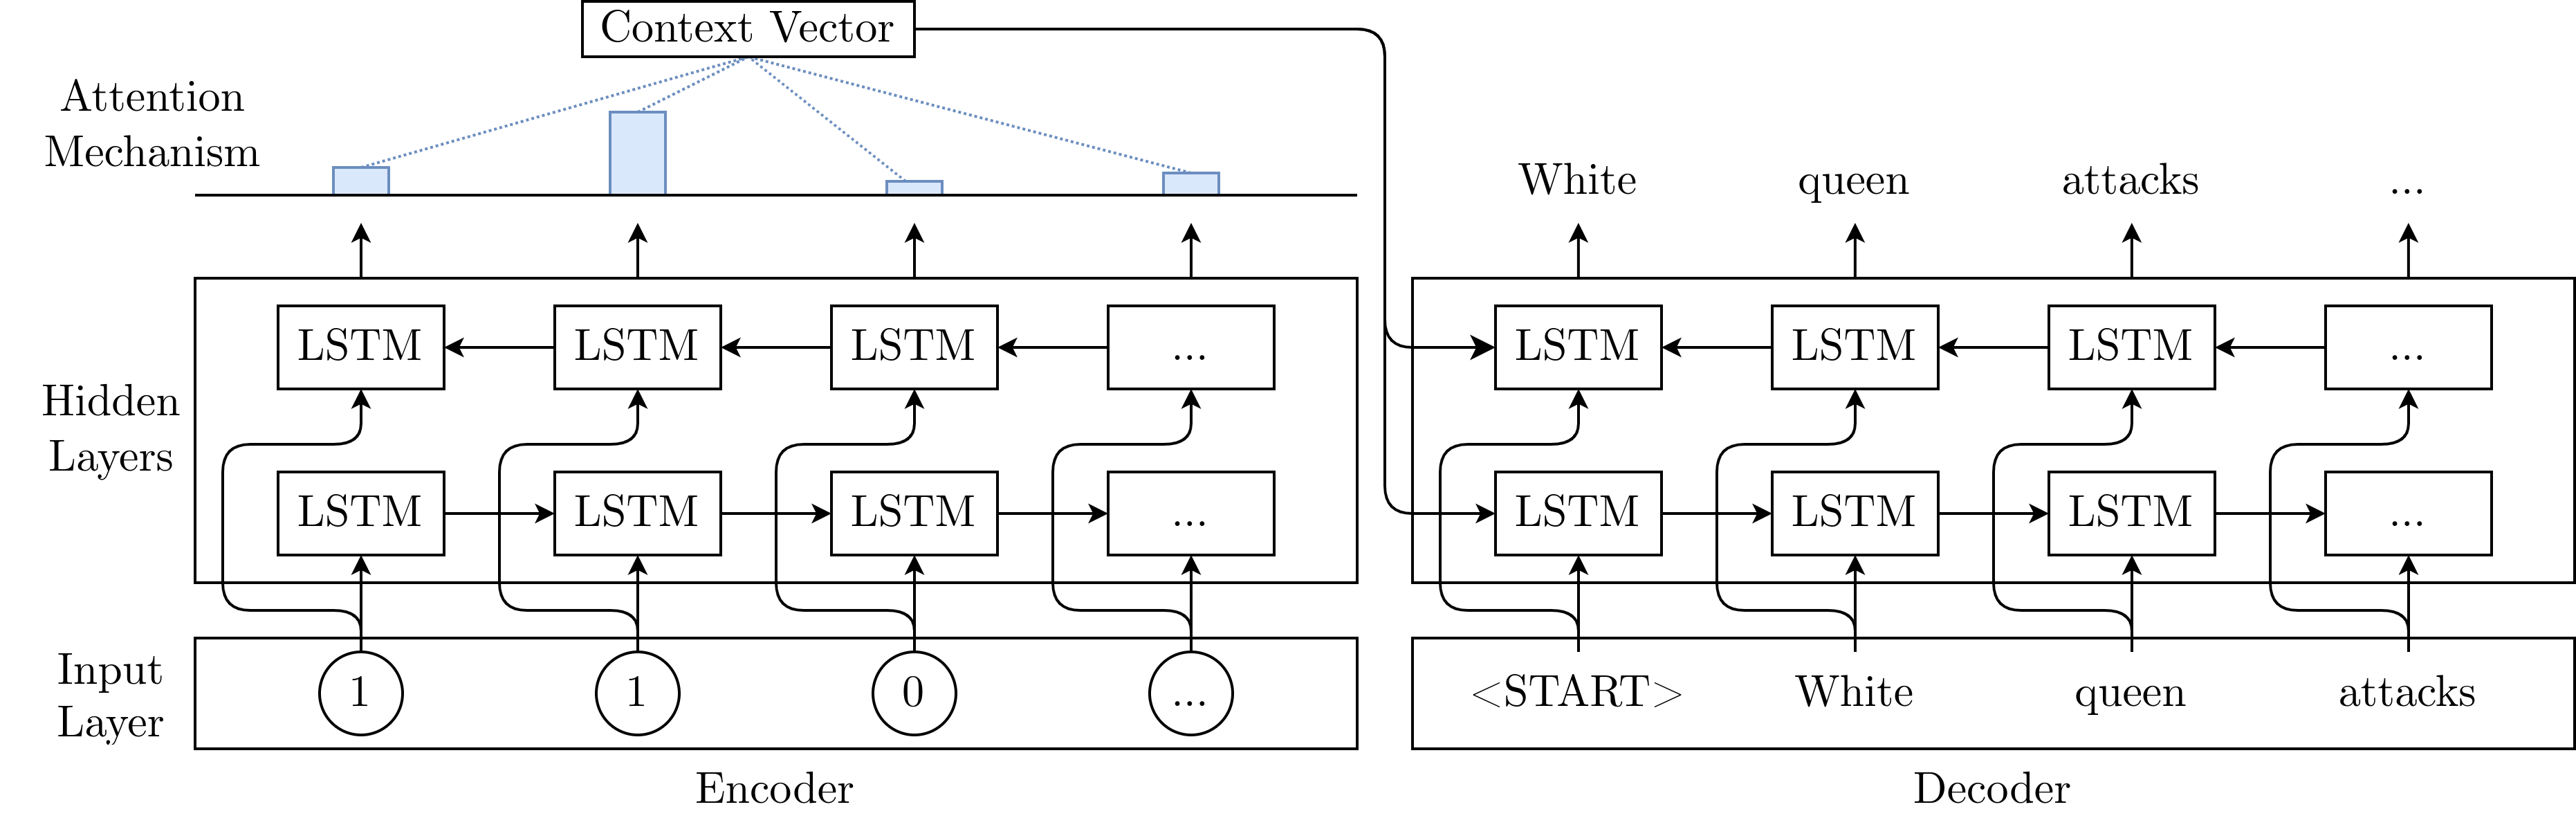
\includegraphics[width=\textwidth]{graphics/commentator_example/general_approach.png}
\caption{Chess Commentator Encoder-Decoder Architecture with Attention Mechanism (Note: Figure based on \cite{jhamtani-etal-2018-learning} Figure 4)}
\label{fig:eda}
\end{figure}

The encoder-decoder architecture used for generating chess commentary makes use of the described Bi-LSTMs.\footnote{Cf. \cite{zang-etal-2019-automated}, p. 2}  It’s a model used in machine translation and other areas of artificial intelligence. It consists of two main components: the encoder and the decoder. The encoder is responsible for converting the input into an appropriate representation (e.g., a vector of numbers). The decoder uses this representation to produce the desired output.\footnote{Cf. \cite{https://doi.org/10.48550/arxiv.1406.1078}, p. 1} In the case of the chess commentary translation the encoder receives a sequence of data, generated by the chess engine (position and move), processes the data and encodes it  into a "fixed-length vector representation"\footnote{\cite{cho-2014-ende}, p. 1}. This vector are the last states of the encoder. The vector can either be used as initialization for the LSTM cells of the decoder or as additional input for each step of the generation of the output.\footnote{Cf. \cite{mohajerin-2017-state}, pp. 1-2} One problem that affects the quality of the decoder’s translation, is the length of the sequences. The sequence stored in the vector tends to dilute over time, resulting in poor translations. To solve it, an attention mechanisms can be used. The attention mechanism allows the decoder to "selectively focusing on parts of the source"\footnote{\cite{luong-2015-attention}, p. 1} while producing the desired output. This is done while processing the data in the encoder, which encodes only the most important information in the vector, called the context vector. It can be said that the context vector contains a summary of the sequence. This allows the decoder to focus only on the information relevant for translation. If the decoder now wants to generate comments, it receives a start symbol as input (represented by \texttt{<START>} in Figure \ref{fig:eda}). This start symbol is used to indicate the start of the output sequence. The first output is the first word of the translation. The output is additionally used as new input in the next step, generates an output and which is used as the new input again. This procedure is repeated until an end symbol is reached, which signals the end of the sequence. The generated output sequence is the translation, so here the chess comments.

\subsubsection{Generation Models}

For a given chess position and a played move, the commentator should create comments on different categories. Those categories are the \textit{description of the current move}, the \textit{description of the move quality}, the \textit{comparison of moves}, the \textit{description of the move planning} and \textit{contextual game information}.\footnote{Cf. Jhamtani et al. 2018 p. 3}$^{,}$\footnote{Cf. Zang et al. 2019, pp. 3-4}

\begin{figure}[h]
\centering
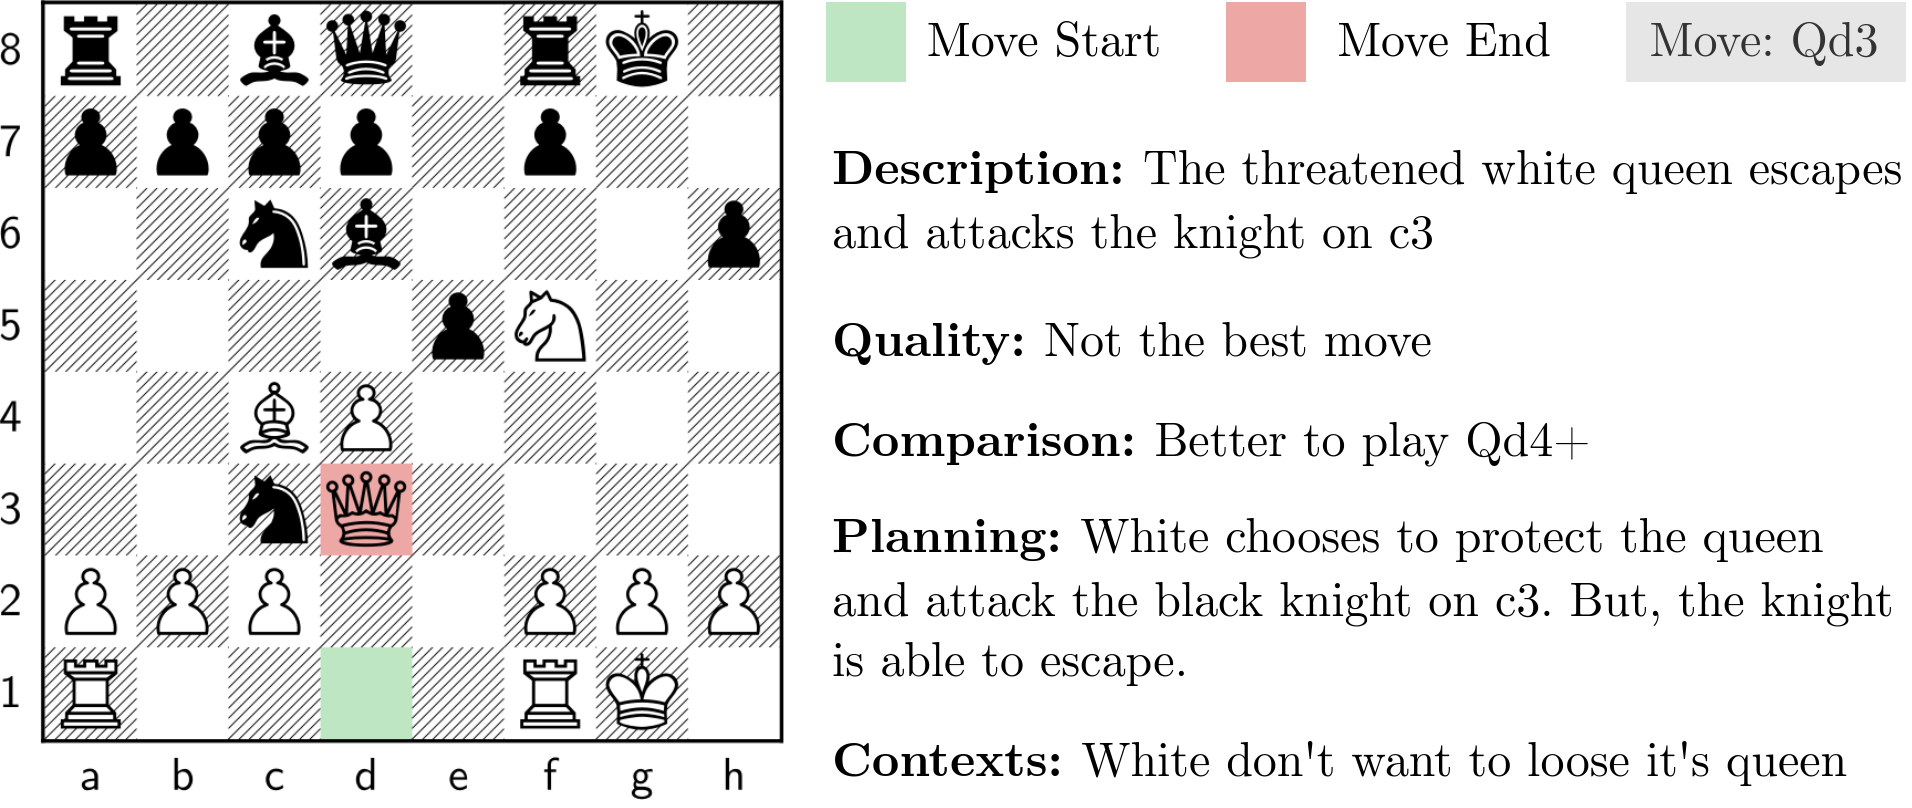
\includegraphics[width=0.7\textwidth]{graphics/commentator_example/commentator.png}
\caption{Chess Commentary Example (Note: Figure based on \cite{zang-etal-2019-automated} Figure 1)}
\end{figure}

Since the procedure for creating comments varies from category to category, it is practically impossible to do this with a single commentator, as simplified described above. Therefore, in the following it will be spoken of five individual ones, each for one of the categories. In addition, instead of categories, it is now spoken of generation models, since these are used to generate comments. These generation models come with two challenges that can have a strong impact on the quality of the generated description: (1) the features on the basis of which the comments for the aspects are generated, (2) the number of moves and the resulting position considered. To overcome the first challenge \cite{jhamtani-etal-2018-learning} used "discrete information (threats, game evaluation scores, etc.)"\footnote{Zang et al. 2019 p. 4}. How \cite{zang-etal-2019-automated} show, those features information did not provide the best results. Therefore, they have used features provided directly by the internal chess engine. These are the \textit{state of the board before the move}, \textit{start square of the move}, \textit{end square of the move}, \textit{piece on the start square}, \textit{piece on the end square}, \textit{promotion state} and  \textit{checking state}. The pieces on the starting square and on the ending square can be different, since the pawns can be replaced by another piece when they reach the opponent's last rank.\footnote{See \cite{fide-2018-loc} p. 6} In this case the promotion state would be set to 1. The advantage of using these features is that they can be easily read from the information provided by the chess engine described in the previous section. The second challenge can be overcome by distinguishing between generation models that need only one move (description and quality) and generation models that need multiple moves (comparision, planning and context) so that the description is accurate. Depending on the model, they implement either a single-move encoder or a multi-move encoder. These two encoders differ in their training so that both can precisely store different amounts of information in the context vector.

% With these challenges overcomed the next steps are

% Once these problems are solved, for each requirement, the information needed to fulfill a requirement must be put into a form that can be used as input, certain features can be easily identified, and the text can be generated based on these identifications.

% In order to generate comments on these requirements, it is necessary to define certain features on the basis of which this is done. \cite{jhamtani-etal-2018-learning} uses features such as, \gls{threats} and position value, but as \cite{zang-etal-2019-automated} show, this information does not consider the following positions well enough, which affects the quality of comments. To solve this problem the requirements were divided into two categories: (1) requirements which need exactly one move to be describe, (2) requirements which need a number of moves to be describe. The second category is only an extension of the first, so the two categories differ in detail only in how many positions and moves they consider; the features included remain the same.

% A method which has shown significant success in the field of natural language processing are Recurrent Neural Networks (RNN).

% The process of generating the text commentary can be summarized into two upper parts, namely encoding and decoding. Encoding describes the extraction and formatting of certain features to make them easier to process, while decoding describes the translation of the encoded features into a text format.

% \subsubsection{Generation Model Types and Feature Emedding}

The generation models can be divided according to the number of moves and positions they consider for the generation. There are models that require only one position and the played move (description and quality), and models that require "multiple moves derived from variations and predictions"\footnote{Zang et al. 2019, pp. 5}. (comparison, planning and context) so that the description is accurate. To implement this, \cite{zang-etal-2019-automated} introduce two types of encoders, a \textit{single-move encoder} and a \textit{multi-move encoder}. The encoders are used to extract and encode certain features from given moves and positions and put them into a format that can it can used by the models for commentary generation.

The single move encoder receives two inputs, a position and the move played, and outputs two encoded vectors. The encoded vectors contain features that are later used as inputs for the neural network. The position received is converted into a representation that can be processed as an input. To generate this representation, the encoder uses the engine, since it has already created an interpretable representation in the form of the BitBoard representation. The move received is examined for various features, which are then encoded in the output vector. Those features are \textit{state of the board before the move}, \textit{start square of the move}, \textit{end square of the move}, \textit{piece on the start square}, \textit{piece on the end square}, \textit{promotion state} and  \textit{checking state}. The pieces on the starting square and on the ending square can be different, since the pawns can be replaced by another piece when they reach the opponent's last rank.\footnote{See \cite{fide-2018-loc} p. 6} In this case the promotion state would be set to true.

$$
sme(p,m) \rightarrow E_p, E_m
$$

\section{Conclusion}

In summary, the research question "how machine learning can be used to generate commentary for chess games" could be answered. However, the problem of the intransparency of moves of professional players and engines remains. Although the models provide good insight, they are not yet capable of providing commentary as insightful as that provided by human commentators. Nevertheless, they show "the direction to further developing"\footnote{\cite{zang-etal-2019-automated}, p. 9}, so that this goal can be achieved in the future with high likelihood. 

% \newpage

% \printnoidxglossaries

\newpage
\addcontentsline{toc}{section}{References}
\bibliographystyle{chicago}
\nocite{*}
\bibliography{references}

\newpage

\begin{center}
\large
\textbf{Declaration of authorship
}\end{center}

\noindent I hereby certify that the following project report was written entirely by me and is based on my work unless otherwise indicated. I am aware of the University's regulations regarding plagiarism, including the following actions in the event of a violation. Any form of use of outside work is identified where appropriate and noted in the sources.

\vspace{1cm}

\begin{center}
\large
Max Semdner
\end{center}

\begin{tabular}{p{5cm}p{10cm}}
& \\
Approved: & \hrulefill \\
& \\
Date: & \hrulefill \\
\end{tabular}

\end{document}

